\section{Results}\label{sec:results}
\subsection{The dispatcher leaks}\label{sec:dispatch}
\begin{table*}[t]\centering\small
\caption{Joint evaluation of the five live policies; 120 test fixtures per row, single host over loopback, synthetic tools. Sel.\ S/A: validation-selected size-only / adaptive attack (primary). Max: largest test count in the frozen suite (descriptive). GMM: label-free removal. Ref.: uniform six-class reference 20/120, or for shadow the realized pair-ambiguity floor (Table~\ref{tab:shadow-floor}). Bytes: whole-connection / call-window factors. Tokens include both planners. Goal and State are separate counts from this cohort; the state-control cohort (Supplement S1) has its own counts.}\label{tab:live-timing-main}
\setlength{\tabcolsep}{4pt}
\begin{tabularx}{\textwidth}{@{}lYrrrrrrr@{}}\toprule
Planner & Policy & Sel. S/A & Max & GMM & Ref. & Bytes$\times$ & Tokens$\times$ & Goal/State \\\midrule

Qwen3:8B & No cover & 117/117 & 117 & -- & 20 & 1.00/1.00 & 1.00 & 113/114 \\
Qwen3:8B & Immediate & 75/112 & 112 & 112 & 20 & 1.15/1.33 & 1.00 & 111/112 \\
Qwen3:8B & History, sequential & 76/93 & 99 & 53 & 20 & 1.15/1.32 & 1.00 & 112/113 \\
Qwen3:8B & History, concurrent & 66/99 & 99 & 38 & 20 & 1.15/1.33 & 1.00 & 111/112 \\
Qwen3:8B & Planner shadow & 54/54 & 70 & 34 & 70.5 & 1.31/1.68 & 2.01 & 112/113 \\
Llama3.1:8B & No cover & 110/110 & 112 & -- & 20 & 1.00/1.00 & 1.00 & 82/70 \\
Llama3.1:8B & Immediate & 80/108 & 108 & 108 & 20 & 1.13/1.27 & 1.01 & 83/67 \\
Llama3.1:8B & History, sequential & 82/104 & 104 & 14 & 20 & 1.13/1.26 & 1.01 & 84/67 \\
Llama3.1:8B & History, concurrent & 68/106 & 106 & 66 & 20 & 1.13/1.27 & 1.02 & 82/67 \\
Llama3.1:8B & Planner shadow & 64/64 & 64 & 43 & 70.5 & 1.35/1.71 & 1.99 & 82/67 \\
\bottomrule\end{tabularx}\end{table*}


\paragraph{Immediate cover is removable}
A label-free two-component mixture over training gaps selects the short-gap component for removal, and a classifier trained on no-cover traffic decodes the rest. On immediate cover this restores 112/120 and 108/120 correct predictions, against selected size-only attacks at 75 and 80 (Table~\ref{tab:live-timing-main}); both gains meet the prespecified replication rule after Holm correction ($p=1.9\times10^{-8}$ and $4.3\times10^{-6}$). Independent TCP reassembly matches all 773,450 recorded TLS record types, lengths and counts, and refitting the mixture on packet-capture clocks reproduces both scores; on held-out immediate calls it flags 181/182 and 182/182 decoys with no false flags (Supplement S2.7). A controller that skips the model wait therefore exposes its cover.

\paragraph{History matching hides the shortcut, not the signal}
Sampling honest gaps defeats the simple mixture: it falls to 53 and 14 (sequential) and 38 and 66 (concurrent). Adapted context removal or joint decoding still recognizes 93/120 and 104/120 sequential executions, against selected size-only attacks at 76 and 82 (Holm $p=.0559$ and $.00078$), and 99/120 and 106/120 concurrent ones against 66 and 68 (both $p<10^{-4}$). The policy controls minimum waits, not achieved timing (Table~\ref{tab:live-draws}): Qwen's mean sampled hold of 40.5\,ms becomes 100.4\,ms sequential and 171.2\,ms concurrent at the record observer.

\begin{table*}[t]\centering\small
\caption{Achieved history-based cover timing, all splits (455 cover calls per row). Means in seconds. An anchor gap is measured from the actual prior completed anchor call to cover record start. Sampled durations are minimum server holds, while achieved durations include record-level transport and scheduling.}
\label{tab:live-draws}
\begin{tabularx}{\textwidth}{@{}lYrrrr@{}}\toprule
Model & Arm & Drawn gap & Achieved anchor gap & Drawn hold & Achieved duration\\\midrule
Qwen & History seq. & 0.5198 & 0.5660 & 0.0405 & 0.1004\\
Qwen & History concurrent & 0.5198 & 0.5772 & 0.0405 & 0.1712\\
Llama & History seq. & 0.5865 & 0.6203 & 0.0768 & 0.1097\\
Llama & History concurrent & 0.5865 & 0.6204 & 0.0768 & 0.1234\\
\bottomrule\end{tabularx}
\end{table*}

 A failed simple attack is therefore not evidence of concealment. Llama's sequential mixture deletes 477/634 honest calls while detecting only 64/182 cover calls, which explains its 14/120, whereas joint decoding on the same traces reaches 104/120.

\subsection{Without call boundaries}\label{sec:noboundary}
We reanalyze all 3,000 episodes from complete encrypted connections, including setup and teardown records. The attacker receives relative record times, directions, ciphertext lengths and destinations, but no call boundaries, operation names, role labels or HTTP stream assignment; whole-episode association remains supplied. An idle-gap rule proposes events (five gaps from 5 to 250\,ms compete on validation accuracy), raw-record classifiers skip eventization, and a training-only mixture removes short-gap events. The immediate-arm pair is the only primary test.

\begin{table}[t]\centering\small
\caption{No supplied call boundaries; whole-episode association remains supplied. B/R: validation-selected idle-grid baseline and removal attacks (primary pair: immediate). Max: largest test count over both suites, including the exploratory protocol-aware eventizer designed after the idle-grid results were seen (descriptive). Counts out of 120; uniform reference 20.}\label{tab:no-call-main}
\setlength{\tabcolsep}{4pt}
\begin{tabularx}{\columnwidth}{@{}Yrrrr@{}}\toprule
 & \multicolumn{2}{c}{Qwen} & \multicolumn{2}{c}{Llama} \\\cmidrule(lr){2-3}\cmidrule(l){4-5}
Policy & B/R & Max & B/R & Max \\\midrule
No cover & 115/109 & 117 & 108/101 & 112 \\
Immediate & 80/69 & 91 & 90/86 & 97 \\
History, sequential & 73/74 & 75 & 88/56 & 93 \\
History, concurrent & 56/61 & 62 & 78/62 & 88 \\
Planner shadow & 69/65 & 73 & 69/56 & 69 \\
\bottomrule\end{tabularx}\end{table}

Selected removal recognizes 69/120 and 86/120 immediate-cover tasks against baselines of 80 and 90, paired differences of $-9.2$ and $-3.3$ points (Holm $p=.025$ and $.54$): the call-window removal advantage does not carry over. An exploratory eventizer, designed after these results were seen, uses the public padding quantum and MCP setup sequence to propose requests; it raises Qwen's removal count from 68 to 91 but lowers Llama's from 90 to 87, and recovers calls poorly (event F1 .295 and .380 at IoU .5). Recognition stays well above the 20/120 reference in every arm (Table~\ref{tab:no-call-main}), so withholding boundaries changes which attack works rather than removing the leak. Because the representations differ, the gap from the call-window counts is not a pure causal effect of boundaries.

\subsection{Planner shadows sit on their floor}\label{sec:shadow}
The strongest tested call-window attack on shadow cover, a size/destination RF, scores 70/120 for Qwen and 64/120 for Llama; the validation-selected attacks score 54 and 64. On the realized test split, 21 of 120 shadow labels match the real one, so the $k=1$ floor of Section~\ref{sec:floor} is 70.5/120. No attack exceeds it: the tested attacks are no more accurate than an attacker who already knew both tasks. A chain-separation attack recovers the real chain exactly in only 29 and 32 fixtures. Record-only attacks give a maximum of 73/120 for Qwen over 52 candidates, 2.5 fixtures above the floor, with selected attacks at 69 and 69 below it.

Whether an attacker can tell the chains apart is a separate question. Among the 99 fixtures whose labels differ, where the floor is one half, aggregate counts bound the forest's real-label accuracy only to $[49,70]/99$ and $[43,64]/99$; the exact test needs per-fixture predictions (Section~\ref{sec:limits}). The prespecified equivalence family is degenerate for shadow because both selectors chose the same attack, and we do not count it. Shadow costs 2.01/1.99 times the model tokens and 1.68/1.71 times the call-window bytes, and raises mean real-chain time from 2.91/3.33\,s to 4.80/3.94\,s.

\subsection{Goal completion misses state}\label{sec:state}
In the live arms, all cover executes on an isolated clone. Goal and state counts stay within three fixtures of no cover for every arm (Table~\ref{tab:live-timing-main}), although cover still changes planning: honest paths match no cover in only 115/120 (Qwen) and 103/120 (Llama) shadow fixtures. Llama's no-cover goal and state counts (82 and 70 of 120) are already imperfect.

The state control tests whether the evaluation would detect forbidden effects. Proxy, read and hidden-isolated cover keep Qwen state correctness at 115--116/120. Live writes reduce it to 7/120 while goal completion stays at 102/120: 95 of the 102 completed tasks leave collateral errors on other orders, shared quota or the ledger. Llama's counts are 3/120 intact and 73 of 76 completed tasks with collateral errors. Both integrity reductions survive Holm correction ($p=3.7\times10^{-32}$ and $3.0\times10^{-19}$; Supplement S1). The harm direction is built into this stress arm; it shows what a goal-only evaluation omits, not how often production writes cause it.

\subsection{Deciding with declared tolerances}\label{sec:decision}
Table~\ref{tab:decision} carries out step 4 of the protocol. The tolerances are illustrative: we set them for this synthetic scenario after the measurements, so the table demonstrates the procedure rather than validating any policy. Against the call-window observer, only the shadow passes, and Llama's shadow does so with its state loss exactly at the limit. Against the record-only observer the picture changes: Qwen's history-concurrent policy passes at no model cost, while Qwen's shadow fails by one fixture. The same measurements thus support different deployments depending on the declared observer and tolerances, which is why the protocol requires both to be fixed before measuring. Tightening the state tolerance to 2/120 fails every Llama arm; loosening inference to 65\% passes Qwen's sequential policy and shadow against the record-only observer. Figure~\ref{fig:frontier} places the measured policies against the derived floors.

\begin{table*}[t]\centering\small
\caption{Protocol step 4 on the live policies under illustrative tolerances, set by us for this synthetic scenario after the measurements and not validated for any deployment: strongest tested recognition $\le 72/120$ (60\%); goal and state each at most 3/120 below no cover; model tokens $\le2.5\times$; call-window bytes $\le2\times$. CW and RO are the call-window and record-only observers (Max counts from Tables~\ref{tab:live-timing-main} and~\ref{tab:no-call-main}). $\Delta$G/$\Delta$S are goal/state differences from no cover. A decision names the first violated tolerance.}\label{tab:decision}
\setlength{\tabcolsep}{4pt}
\begin{tabularx}{\textwidth}{@{}llrrrrrYY@{}}\toprule
Planner & Policy & CW Max & RO Max & $\Delta$G/$\Delta$S & Tokens$\times$ & Bytes$\times$ & Decision, CW observer & Decision, RO observer \\\midrule
Qwen3:8B & Immediate & 112 & 91 & $-2$/$-2$ & 1.00 & 1.33 & Fail: inference & Fail: inference \\
Qwen3:8B & History, sequential & 99 & 75 & $-1$/$-1$ & 1.00 & 1.32 & Fail: inference & Fail: inference (by 3) \\
Qwen3:8B & History, concurrent & 99 & 62 & $-2$/$-2$ & 1.00 & 1.33 & Fail: inference & \textbf{Pass} \\
Qwen3:8B & Planner shadow & 70 & 73 & $-1$/$-1$ & 2.01 & 1.68 & \textbf{Pass} & Fail: inference (by 1) \\\midrule
Llama3.1:8B & Immediate & 108 & 97 & $+1$/$-3$ & 1.01 & 1.27 & Fail: inference & Fail: inference \\
Llama3.1:8B & History, sequential & 104 & 93 & $+2$/$-3$ & 1.01 & 1.26 & Fail: inference & Fail: inference \\
Llama3.1:8B & History, concurrent & 106 & 88 & $0$/$-3$ & 1.02 & 1.27 & Fail: inference & Fail: inference \\
Llama3.1:8B & Planner shadow & 64 & 69 & $0$/$-3$ & 1.99 & 1.71 & \textbf{Pass} (state at limit) & \textbf{Pass} (state at limit) \\\bottomrule
\end{tabularx}\end{table*}

\begin{figure}[t]\centering
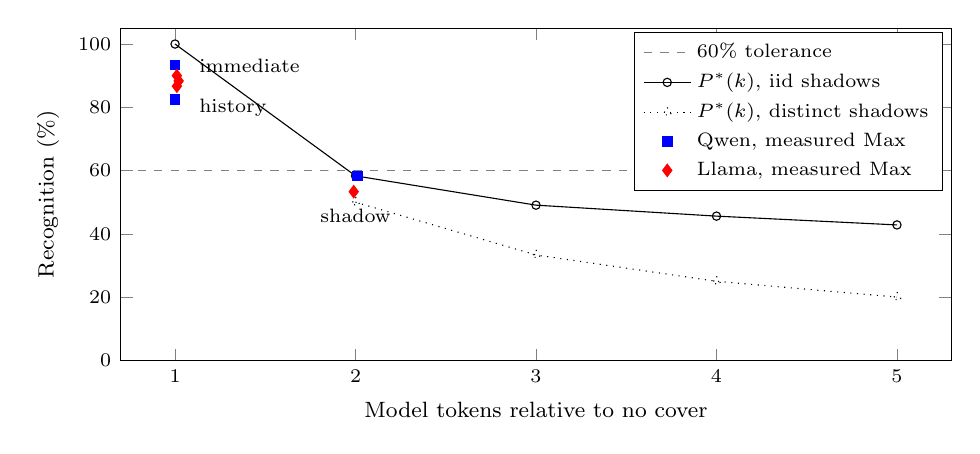
\begin{tikzpicture}
\begin{axis}[width=\columnwidth,height=5.8cm,xmin=0.7,xmax=5.3,ymin=0,ymax=105,
 xlabel={Model tokens relative to no cover},ylabel={Recognition (\%)},
 xtick={1,2,3,4,5},ytick={0,20,40,60,80,100},
 legend style={font=\scriptsize,at={(0.99,0.99)},anchor=north east,cells={anchor=west}},
 tick label style={font=\scriptsize},label style={font=\footnotesize}]
\addplot[gray,dashed,mark=none,domain=0.7:5.3] {60};
\addlegendentry{60\% tolerance}
\addplot[black,mark=o,mark size=1.5pt] coordinates {(1,100) (2,58.33) (3,49.07) (4,45.60) (5,42.82)};
\addlegendentry{$P^*(k)$, iid shadows}
\addplot[black,dotted,mark=triangle,mark size=1.8pt] coordinates {(2,50) (3,33.33) (4,25) (5,20)};
\addlegendentry{$P^*(k)$, distinct shadows}
\addplot[only marks,blue,mark=square*,mark size=1.7pt] coordinates {(1,93.33) (1,82.5) (1,82.5) (2.01,58.33)};
\addlegendentry{Qwen, measured Max}
\addplot[only marks,red,mark=diamond*,mark size=2.2pt] coordinates {(1.01,90) (1.01,86.67) (1.02,88.33) (1.99,53.33)};
\addlegendentry{Llama, measured Max}
\node[font=\scriptsize,anchor=west] at (axis cs:1.08,93) {immediate};
\node[font=\scriptsize,anchor=west] at (axis cs:1.08,80) {history};
\node[font=\scriptsize,anchor=north] at (axis cs:2,51) {shadow};
\end{axis}
\end{tikzpicture}
\caption{Inference--cost frontier against the call-window observer. Points are the strongest tested attacks for the four cover arms; lines are the derived pair-ambiguity floors for $k=0$--4 shadows. Only $k=1$ with iid labels was measured. Controller cover costs no model work but leaves 83--93\% recognition; the measured shadow sits on its floor.}\label{fig:frontier}
\end{figure}

